\documentclass[a4paper]{article}
\usepackage{a4wide}
\usepackage{graphicx}
\usepackage{pxfonts}
\usepackage{tikz}
\usepackage{calc}
\usepackage{ifthen}
\usepackage{listings}
\usepackage{url}
\usepackage{booktabs}

\usetikzlibrary{calc,decorations.text,patterns,shapes.arrows,shapes,shadings,arrows,automata,positioning,shadows}

\pgfkeys{/tikz/flowchart/node/.style={rectangle,fill=blue,opacity=0.5,text opacity=1,drop shadow,inner sep=2mm}}
\pgfkeys{/tikz/flowchart/arrow/.style={-latex,thick}}
\pgfkeys{/tikz/flowchart/arrowline/.style={thick}}

\pagestyle{empty}

\newcommand{\PLACEHOLDER}[1]{\ensuremath{\langle}\textrm{\textit{#1}\ensuremath{\rangle}}}
\newcommand{\X}[2]{\tikz[baseline,remember picture]{\node[anchor=base,inner sep=0mm] (#2) {{#1}};}}

\lstdefinelanguage{generic}{
  escapechar=@,%
  basicstyle={\ttfamily},%
  keywordstyle={\ttfamily\bfseries},%
  commentstyle={\it},%
  frame=lines,%
  captionpos=b%
}

\lstdefinelanguage{javascript}[]{generic}{%  
  morekeywords={function,var,if,for,while,break,do,delete,in,instanceof,new,return,this,switch,throw,try,catch,typeof,int,void,with,yield,label,import,export,continue,true,false},%
  escapechar=@,%
  basicstyle={\ttfamily},%
  keywordstyle={\ttfamily\bfseries},%
  commentstyle={\it},%
  frame=lines,%
  captionpos=b,%
  sensitive=true,%
  morecomment=[l]{//},%
  morecomment=[s]{/*}{*/},%
  morestring=[b]",%
  moredelim=**[is][\color{red}]{\#}{\#}%
}

\lstdefinelanguage{HTML}[]{generic}{
    morecomment = [l]{//},
    morecomment = [l]{///},
    morecomment = [s]{/*}{*/},
    morestring=[b]",
    sensitive = true,
    captionpos=b,
    morekeywords = {html, head, body, script, title}
}

\lstdefinelanguage{MyJava}[]{java}{
  escapechar=@,%
  basicstyle={\ttfamily},%
  keywordstyle={\ttfamily\bfseries},%
  commentstyle={\it},%
}

\newcommand{\examplecode}[2][javascript]{\begin{center}\begin{minipage}{.9\linewidth}\lstinputlisting[language=#1]{#2}\end{minipage}\end{center}}

\renewcommand{\section}[1]{
  \begin{center}
    \Huge\sc #1
  \end{center}
}
\renewcommand{\subsection}[1]{
  \begin{center}
    \Large\sc #1
  \end{center}
}

\begin{document}

\begin{center}
  \Huge Java Cheat Sheet
\end{center}

\section{Primitieve Types}
\begin{center}
  \begin{tabular}{lll}
    {\bf Gehele getallen} & {\tt byte} & -128 \dots 127 \\ \cmidrule{2-3}
                          & {\tt short} & -32,768 \dots 32767 \\ \cmidrule{2-3}
                          & {\tt\bfseries int} & -2,147,483,648 \dots 2,147,483,647 \\ \cmidrule{2-3}
                          & {\tt long} & $-2^{63} \dots 2^{63}-1$ \\
    \midrule
    {\bf Kommagetallen} & {\tt float} & $1.4 \times 10^{-45} \dots 3.4 \times 10^{38}$ \\ \cmidrule{2-3}
                        & {\tt\bfseries double} & $4.9 \times 10^{-324} \dots 1.8 \times 10^{308}$ \\
    \midrule
    {\bf Booleaanse waarden} & {\tt\bfseries boolean} & {\tt true}, {\tt false} \\
    \midrule
    {\bf Tekens}        & {\tt\bfseries char} & {\tt 'a'}, {\tt 'b'}, {\tt '+'}, {\tt '?'}, \dots
  \end{tabular}
\end{center}

\vfil

\section{Naamgeving}
\begin{center}
  \begin{tabular}{ll}
    Type identifier & Conventie \\
    \toprule
    Klasse & {\bf U}pper{\bf C}amel{\bf C}ase \\
    Interface & {\bf U}pper{\bf C}amel{\bf C}ase \\
    Methode & {\bf l}ower{\bf C}amel{\bf C}ase \\
    Variabele & {\bf l}ower{\bf C}amel{\bf C}ase \\
  \end{tabular}
\end{center}

\vfil

\section{Operaties}
\subsection{Rekenkundige Operaties}
\begin{center}
  \begin{tabular}{cl}
    {\bf Operator} & {\bf Omschrijving} \\
    \toprule
    {\tt +} & Optelling \\
    {\tt -} & Aftrekking \\
    {\tt *} & Vermenigvuldiging \\
    {\tt /} & Deling \\
    {\tt \%} & Modulo \\
  \end{tabular}
\end{center}

\subsection{Logische Operatoren}
\begin{center}
  \begin{tabular}{cl}
    {\bf Operator} & {\bf Omschrijving} \\
    \toprule
    {\tt \&\&} & And \\
    {\tt ||} & Or \\
    {\tt !} & Not \\
  \end{tabular}
\end{center}

\begin{samepage}
\section{Control Flow}
\vfil
\subsection{{\tt if}-statement}
\begin{center}
  \begin{minipage}{.45\textwidth}
    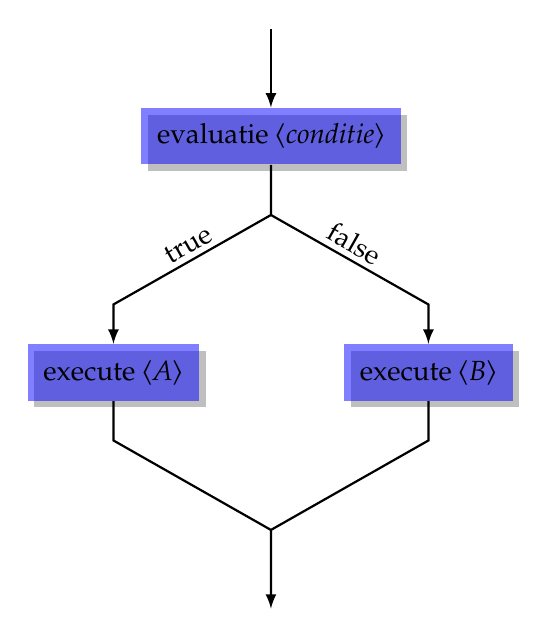
\begin{tikzpicture}
  \node[flowchart/node] (if) at (0,3) {evaluatie \PLACEHOLDER{conditie}};
  \node[flowchart/node] (then) at (-2, 0) {execute \PLACEHOLDER{A}};
  \node[flowchart/node] (else) at (2, 0) {execute \PLACEHOLDER{B}};

  \draw[flowchart/arrow] ($ (if.north) + (0,1) $) -- (if.north);
  \draw[flowchart/arrow] (if.south) -- (0,2) -- ($ (then.north) + (0,0.5) $) -- (then.north);
  \draw[flowchart/arrow] (0,2) -- ($ (else.north) + (0,0.5) $) -- (else.north);
  \path[flowchart/arrow,decorate,decoration={text along path,text={true},text align={align=center},reverse path}] (0, 2.1) -- ($ (then.north) + (0,0.6) $);
  \path[flowchart/arrow,decorate,decoration={text along path,text={false},text align={align=center}}] (0, 2.1) -- ($ (else.north) + (0,0.6) $);

  \draw[flowchart/arrow] (then.south) -- ($ (then.south) - (0,0.5) $) -- (0,-2) -- (0,-3);
  \draw[flowchart/arrowline] (else.south) -- ($ (else.south) - (0,0.5) $) -- (0,-2);
\end{tikzpicture}

  \end{minipage}
  \hspace{4mm}
  \begin{minipage}{.3\textwidth}
    \examplecode[MyJava]{if.java}
  \end{minipage}
\end{center}
\end{samepage}

\vfil

\begin{samepage}
\subsection{{\tt while}-lus}
\begin{center}
  \begin{minipage}{.45\textwidth}
    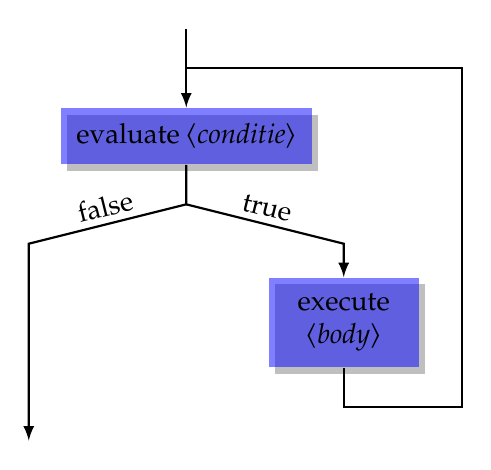
\begin{tikzpicture}
  \node[flowchart/node] (while) {evaluate \PLACEHOLDER{conditie}};
  \node (loop entry) at ($ (while.north) + (0,0.5) $) {};
  \node[flowchart/node] (body) at ($ (while.south) + (2,-2) $) {\parbox{1.5cm}{\centering execute \PLACEHOLDER{body}}};
  \node (split) at ($ (while.south) + (0,-0.5) $) {};

  \draw[flowchart/arrow] ($ (while.north) + (0,1) $) -- (while.north);
  \draw[flowchart/arrow] (while.south) -- (split.center) -- ++(-2,-0.5) -- ++(0,-2.5);
  \draw[flowchart/arrow] (split.center) -- ++(2,-0.5) -- (body.north);
  \draw[flowchart/arrowline] (body.south) -- ++(0,-0.5) -- ++(1.5,0) |- (loop entry.center);

  \path[flowchart/arrow,decorate,decoration={text along path,text={false},text align={align=center},reverse path}] ($ (while.south) + (0,-0.4) $) -- ++(-2,-0.5);
  \path[flowchart/arrow,decorate,decoration={text along path,text={true},text align={align=center}}] ($ (while.south) + (0,-0.4) $) -- ++(2,-0.5);
\end{tikzpicture}

  \end{minipage}
  \hspace{4mm}
  \begin{minipage}{.3\textwidth}
    \examplecode[MyJava]{while.java}
  \end{minipage}
\end{center}
\end{samepage}

\clearpage

\begin{samepage}
\subsection{{\tt for}-lus}
\begin{center}
  \begin{minipage}{.45\textwidth}
    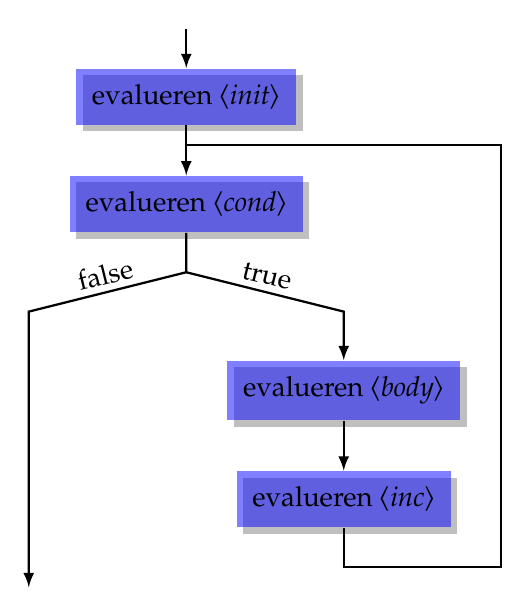
\begin{tikzpicture}
  \node[flowchart/node] (init) {evalueren \PLACEHOLDER{init}};
  \node (loop) at ($ (init.south) + (0,-0.25) $) {};
  \node[flowchart/node] (cond) at ($ (init.south) + (0,-1) $) {evalueren \PLACEHOLDER{cond}};
  \node (split) at ($ (cond.south) + (0,-0.5) $) {};
  \node[flowchart/node] (body) at ($ (split.center) + (2,-1.5) $) {evalueren \PLACEHOLDER{body}};
  \node[flowchart/node] (inc) at ($ (body.south) + (0,-1) $) {evalueren \PLACEHOLDER{inc}};

  \draw[flowchart/arrow] ($ (init.north) + (0,0.5) $) -- (init.north);
  \draw[flowchart/arrow] (init.south) -- (cond.north);
  \draw[flowchart/arrow] (cond.south) -- (split.center) -- ++(-2,-0.5) -- ++(0,-3.5);
  \draw[flowchart/arrow] (split.center) -- ++(2,-0.5) -- (body.north);
  \draw[flowchart/arrow] (body.south) -- (inc.north);
  \draw[flowchart/arrowline] (inc.south) -- ++(0,-0.5) -- ++(2,0) |- (loop.center);

  \path[flowchart/arrow,decorate,decoration={text along path,text={false},text align={align=center},reverse path}] ($ (split.center) + (0,.1) $) -- ++(-2,-0.5);
  \path[flowchart/arrow,decorate,decoration={text along path,text={true},text align={align=center}}] ($ (split.center) + (0,.1) $) -- ++(2,-0.5);
\end{tikzpicture}

  \end{minipage}
  \hspace{4mm}
  \begin{minipage}{.3\textwidth}
    \examplecode[MyJava]{for.java}
    is equivalent met
    \examplecode[MyJava]{foraswhile.java}
  \end{minipage}
\end{center}
\end{samepage}

\vfill
\section{Arrays}
\begin{center}
  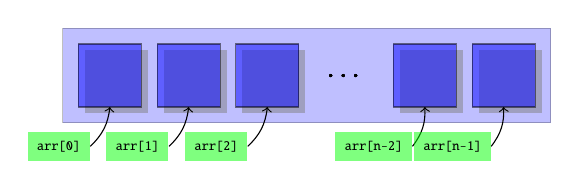
\begin{tikzpicture}[cell/.style={drop shadow,fill=blue,opacity=.5},
                      array/.style={fill=blue,opacity=.25},
                      index/.style={fill=green,opacity=.5,text opacity=1},
                      arr/.style={->}]
    \draw[array] (-0.2,-0.2) rectangle (6,1);
    \foreach \x/\idx in {0/arr[0],1/arr[1],2/arr[2],4/arr[n-2],5/arr[n-1]} {
      \draw[cell] (\x,0) rectangle ($ (\x, 0) + (0.8, 0.8) $);
      \node[index] (node\x) at ($ (\x, 0) - (0.25,.5) $) { {\tt\tiny \idx} };
      \draw[arr] (node\x.east) to [bend right=20] ($ (\x, 0) + (.4,0) $);
      \node at (3.4,0.4) { \dots };
    }

  \end{tikzpicture}
\end{center}

\begin{center}
  \begin{tabular}{p{6cm}l}
    {\bf Operatie} & {\bf Code} \\
    \toprule
    \raggedright Aanmaak array met plaats voor {\tt n} waarden van type {\tt T} & {\tt T[] arr = new T[n];} \\
    \midrule
    \raggedright Opvragen lengte array & {\tt int len = arr.length;} \\
    \midrule
    {\raggedright Uitlezen element op index {\tt i}} & {\tt x = arr[i];} \\
    \midrule
    \raggedright Schrijven naar index {\tt i} & {\tt arr[i] = x;} \\
  \end{tabular}
\end{center}

\vfill

\clearpage
\section{Klassen}
\subsection{Klasse}

\examplecode[MyJava]{class.java}

\begin{tikzpicture}[overlay,
                    remember picture,
                    box/.style={fill=green,opacity=.25},
                    annot/.style={fill=blue,opacity=.25,text opacity=1},
                    empty/.style={},
                    arr/.style={->}]
  \coordinate (class upper left) at ($ (class.north west) + (-0.1,0.1) $);
  \coordinate (class lower right) at ($ (class.south east) + (0.1,-0.1) $) {};
  \coordinate (class upper right) at ($ (class.north east) + (0.1,0.1) $) {};

  \coordinate (fields upper right) at ($ (fieldfirst.north east) + (0.1,0.1) $);
  \coordinate (fields lower left) at ($ (fieldlast.south west) + (-0.1,-0.1) $);

  \coordinate (constructor upper right) at ($ (constructorbegin.north east) + (0.1,0.1) $);
  \coordinate (constructor lower left) at ($ (constructorend.south west) + (-0.1,-0.1) $);

  \coordinate (methods lower left) at ($ (methodbottom.south west) + (-0.1,-0.1) $);
  \path let \p1=(methodtop.north), \p2=(methodright.east) in coordinate (methods upper right) at ($ (\x2, \y1) + (0.1, 0.1) $);
  \coordinate (methods lower left) at ($ (methodbottom.south west) + (-0.1, -0.1) $);

  \draw[box] (class upper left) rectangle (class lower right);
  \draw[box] (fields upper right) rectangle (fields lower left) ;
  \draw[box] (constructor upper right) rectangle (constructor lower left) ;
  \draw[box] (methods upper right) rectangle (methods lower left) ;

  \node[annot,anchor=west] (class annot) at ($ (class upper right) + (0.5, 0.2) $) {\tiny klassenaam};
  \draw[arr] (class annot.west) to [bend right=30] (class upper right);

  \node[annot,anchor=west] (fields annot) at ($ (fields upper right.north east) + (0.5, 0.2) $) {\tiny velden};
  \draw[arr] (fields annot.west) to [bend right=30] (fields upper right);

  \node[annot,anchor=west] (constructor annot) at ($ (constructor upper right) + (0.5, 0.2) $) {\tiny constructor};
  \draw[arr] (constructor annot.west) to [bend right=30] (constructor upper right);

  \node[annot,anchor=west] (methods annot) at ($ (methods upper right) + (0.5, 0.2) $) {\tiny methodes};
  \draw[arr] (methods annot.west) to [bend right=30] (methods upper right);
\end{tikzpicture}


\subsection{Veld}

\begin{center}
  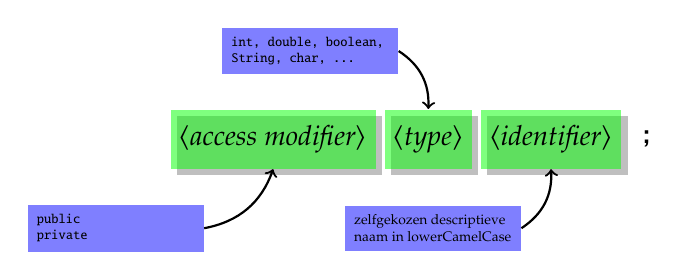
\begin{tikzpicture}[keyword/.style={rectangle,opacity=0.5,text opacity=1,fill=green,minimum height=0.75cm,drop shadow},
                      note/.style={rectangle,opacity=0.5,text opacity=1,fill=blue},
                      arrow/.style={->,thick}]
    \node[keyword] (access modifier) {\PLACEHOLDER{access modifier}};
    \node[keyword,anchor=west,xshift=1mm] (type) at (access modifier.east) {\PLACEHOLDER{type}};
    \node[keyword,anchor=west,xshift=1mm] (identifier) at (type.east) {\PLACEHOLDER{identifier}};
    \node[anchor=west,xshift=1mm] (semicolon) at (identifier.east) {{\tt ;}};

    \node[note] (access modifier note) at ($ (access modifier.south) + (-2,-.75) $) {\parbox{2cm}{\tt\tiny public \\ private}};
    \node[note] (type note) at ($ (type.south) + (-1.5,1.5) $) {\parbox{2cm}{\tt\tiny int, double, boolean, String, char, \dots}};
    \node[note] (identifier note) at ($ (identifier.south) + (-1.5,-.75) $) {\parbox{2cm}{\tiny\raggedright zelfgekozen descriptieve naam in lowerCamelCase}};

    \draw[arrow] (access modifier note.east) to [bend right=30] (access modifier.south);
    \draw[arrow] (type note.east) to [bend left=30] (type.north);
    \draw[arrow] (identifier note.east) to [bend right=30] (identifier.south);
  \end{tikzpicture}
\end{center}

\subsection{Constructor}
\begin{center}
  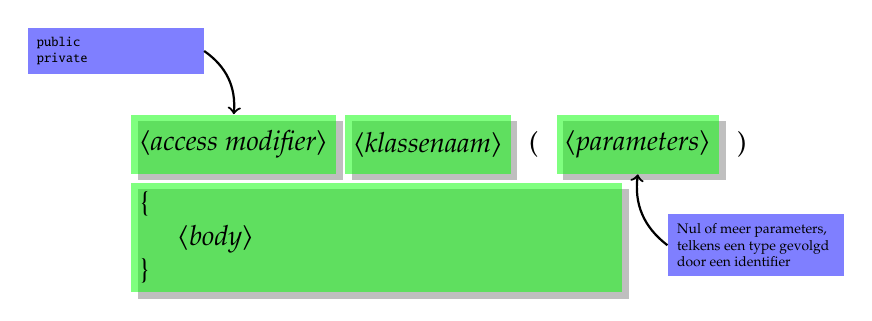
\begin{tikzpicture}[keyword/.style={rectangle,opacity=0.5,text opacity=1,fill=green,minimum height=0.75cm,drop shadow},
                      note/.style={rectangle,opacity=0.5,text opacity=1,fill=blue},
                      arrow/.style={->,thick}]
    \node[keyword] (access modifier) {\PLACEHOLDER{access modifier}};
    \node[keyword,anchor=west,xshift=1mm] (identifier) at (access modifier.east) {\PLACEHOLDER{klassenaam}};
    \node[anchor=west,xshift=1mm] (lparen) at (identifier.east) {(};
    \node[keyword,anchor=west,xshift=1mm] (parameters) at (lparen.east) {\PLACEHOLDER{parameters}};
    \node[anchor=west,xshift=1mm] (rparen) at (parameters.east) {)};
    \node[keyword,anchor=north west,yshift=-1mm] (body) at (access modifier.south west) {\parbox{6cm}{\{ \\ \hspace*{4mm} \PLACEHOLDER{body} \\ \}}};

    \node[note,anchor=south] (access modifier note) at ($ (access modifier.north) + (-1.5,.5) $) {\parbox{2cm}{\tt\tiny public \\ private}};
    \node[note,anchor=north] (parameters note) at ($ (parameters.south) + (1.5,-.5) $) {\parbox{2cm}{\tiny\raggedright Nul of meer parameters, telkens een type gevolgd door een identifier}};

    \draw[arrow] (access modifier note.east) to [bend left=30] (access modifier.north);
    \draw[arrow] (parameters note.west) to [bend left=30] (parameters.south);
  \end{tikzpicture}
\end{center}

\subsection{Methode}
\begin{center}
  \begin{tikzpicture}[keyword/.style={rectangle,opacity=0.5,text opacity=1,fill=green,minimum height=0.75cm,drop shadow},
                      note/.style={rectangle,opacity=0.5,text opacity=1,fill=blue},
                      arrow/.style={->,thick}]
    \node[keyword] (access modifier) {\PLACEHOLDER{access modifier}};
    \node[keyword,anchor=west,xshift=1mm] (return type) at (access modifier.east) {\PLACEHOLDER{type}};
    \node[keyword,anchor=west,xshift=1mm] (identifier) at (return type.east) {\PLACEHOLDER{identifier}};
    \node[anchor=west,xshift=1mm] (lparen) at (identifier.east) {(};
    \node[keyword,anchor=west,xshift=1mm] (parameters) at (lparen.east) {\PLACEHOLDER{parameters}};
    \node[anchor=west,xshift=1mm] (rparen) at (parameters.east) {)};
    \node[keyword,anchor=north west,yshift=-1mm] (body) at (access modifier.south west) {\parbox{6cm}{\{ \\ \hspace*{4mm} \PLACEHOLDER{body} \\ \}}};

    \node[note,anchor=south] (access modifier note) at ($ (access modifier.north) + (-1.5,.5) $) {\parbox{2cm}{\tt\tiny public \\ private}};
    \node[note,anchor=south] (type note) at ($ (type.north) + (0,.5) $) {\parbox{2cm}{\tt\tiny int, double, boolean, String, char, \dots}};
    \node[note,anchor=south] (identifier note) at ($ (identifier.north) + (1.5,.5) $) {\parbox{2cm}{\tt\tiny\raggedright Descriptieve naam in lowerCamelCase}};
    \node[note,anchor=north] (parameters note) at ($ (parameters.south) + (1.5,-.5) $) {\parbox{2cm}{\tiny\raggedright Nul of meer parameters, telkens een type gevolgd door een identifier}};

    \draw[arrow] (access modifier note.east) to [bend left=30] (access modifier.north);
    \draw[arrow] (type note.south) to [bend left=30] (type.north);
    \draw[arrow] (identifier note.west) to [bend right=30] (identifier.north);
    \draw[arrow] (parameters note.west) to [bend left=30] (parameters.south);
  \end{tikzpicture}
\end{center}


\end{document}